\documentclass[12pt,a4paper]{article}

% ─── Packages ──────────────────────────────────────────────────────────────────
\usepackage[margin=2.5cm]{geometry}
\usepackage{graphicx}
\usepackage{amsmath}
\usepackage{amssymb}
\usepackage{booktabs}
\usepackage{multirow}
\usepackage{float}
\usepackage{xcolor}
\usepackage{listings}
\usepackage{caption}
\usepackage{subcaption}
\usepackage{hyperref}
\usepackage{tikz}
\usepackage{pgfplots}
\usepackage{pgfplotstable}
\usepackage{mdframed}
\pgfplotsset{compat=1.18}
\usetikzlibrary{arrows.meta, positioning, shapes.geometric, fit, backgrounds,
                decorations.pathreplacing, calc, matrix, chains, scopes,
                patterns, decorations.markings}

% ─── Colour palette ────────────────────────────────────────────────────────────
\definecolor{serialcol}{RGB}{70,130,180}
\definecolor{ompcol}{RGB}{34,139,34}
\definecolor{posixcol}{RGB}{210,105,30}
\definecolor{mpicol}{RGB}{148,0,211}
\definecolor{cudacol}{RGB}{220,20,60}
\definecolor{hybridcol}{RGB}{0,139,139}
\definecolor{lightgray}{RGB}{230,230,230}
\definecolor{darkgray}{RGB}{80,80,80}
\definecolor{tileA}{RGB}{173,216,230}
\definecolor{tileB}{RGB}{144,238,144}
\definecolor{tileC}{RGB}{255,228,181}
\definecolor{tileD}{RGB}{255,182,193}
\definecolor{seambg}{RGB}{255,200,200}
\definecolor{warncol}{RGB}{180,0,0}

% ─── Listing style ─────────────────────────────────────────────────────────────
\lstset{
  basicstyle=\ttfamily\footnotesize,
  breaklines=true,
  frame=single,
  backgroundcolor=\color{lightgray},
  keywordstyle=\color{blue}\bfseries,
  commentstyle=\color{darkgray}\itshape,
  numbers=left, numberstyle=\tiny\color{gray}, numbersep=6pt,
  tabsize=4
}

% ─── Hyperref ──────────────────────────────────────────────────────────────────
\hypersetup{colorlinks=true, linkcolor=blue, citecolor=blue, urlcolor=blue}

% ─── Note box ──────────────────────────────────────────────────────────────────
\newmdenv[linecolor=warncol,backgroundcolor=seambg!40,
          leftmargin=0pt,rightmargin=0pt,
          innertopmargin=4pt,innerbottommargin=4pt]{notebox}

% ═══════════════════════════════════════════════════════════════════════════════
\begin{document}

% ─── Title ─────────────────────────────────────────────────────────────────────
\begin{titlepage}
  \centering
  \vspace*{2cm}
  {\Huge\bfseries Parallel Image Convolution\\[0.4em]
   \Large Analysis Report\par}
  \vspace{1.5cm}
  {\large High Performance Computing (HPC)\\[0.3em]
   7th Semester --- BSc.\ Engineering\par}
  \vspace{2cm}
  \begin{tabular}{ll}
    \textbf{Implementations:} & Serial, OpenMP, POSIX Pthreads, MPI, CUDA, MPI+OpenMP \\[4pt]
    \textbf{Filters Tested:}  & Gaussian Blur, Edge Detection, Sharpen \\[4pt]
    \textbf{Repository:}      & Parallel-Image-Convolution \\[4pt]
    \textbf{Date:}            & May 2026 \\
  \end{tabular}
  \vfill
  {\large\bfseries Team Members\par}
  \vspace{0.5cm}
  Imalsha Ranasinghe\\
\end{titlepage}

% ─── Table of Contents ─────────────────────────────────────────────────────────
\tableofcontents
\newpage

% ═══════════════════════════════════════════════════════════════════════════════
\section{Introduction}

Image convolution is a fundamental operation in computer vision and image
processing. Given an input image $I$ and a convolution kernel $K$ of size
$k \times k$, the output pixel at position $(x,y)$ and colour channel $c$ is:

\begin{equation}
  O(x,y,c) \;=\;
  \sum_{ky=-\lfloor k/2\rfloor}^{\lfloor k/2\rfloor}
  \sum_{kx=-\lfloor k/2\rfloor}^{\lfloor k/2\rfloor}
  I\!\left(\text{clamp}(x+kx,0,W{-}1),\,
           \text{clamp}(y+ky,0,H{-}1),\,c\right)
  \cdot K(kx,ky)
  \label{eq:conv}
\end{equation}

For a $W \times H$ image with $C$ channels, Eq.~\eqref{eq:conv} requires
$W \cdot H \cdot C \cdot k^2$ multiply-accumulate operations. For our Gaussian
blur kernel ($k=21$, $k^2=441$) on a $2000\!\times\!1333$ image with $C=3$
channels this is $\approx\!3.5\times10^9$ operations --- clearly motivating
parallelism.

This report describes five parallel implementations (OpenMP, POSIX Pthreads,
MPI, CUDA, and a Hybrid MPI+OpenMP approach), analyses their correctness
relative to the serial baseline using Root Mean Square Error (RMSE), and
benchmarks execution time as a function of the degree of parallelism.

% ═══════════════════════════════════════════════════════════════════════════════
\section{Parallel Programming Concepts Applied}

\subsection{Overview of the Parallelisation Strategy}

All parallel implementations exploit the \emph{embarrassingly parallel} nature
of 2D convolution: each output pixel is computed independently, depending only
on a fixed-size neighbourhood of \emph{read-only} input pixels. No inter-pixel
communication is needed during computation; only load balancing and result
assembly require coordination.

The dominant decomposition is \textbf{row-block partitioning}: the image rows
are divided into contiguous chunks and assigned to parallel workers (threads or
processes), ensuring each worker accesses a contiguous memory region and
maximising cache locality.

\begin{figure}[H]
\centering
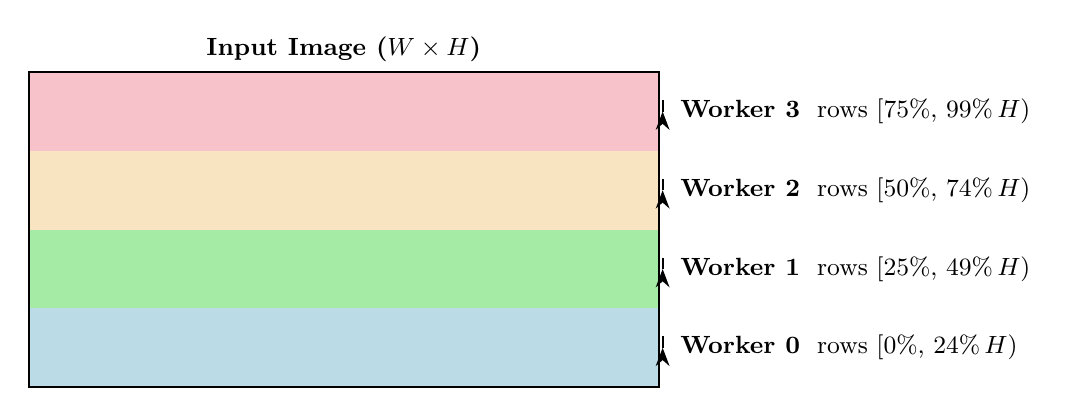
\begin{tikzpicture}[font=\small]
  \node[draw, fill=lightgray, minimum width=8cm, minimum height=4cm,
        label=above:\textbf{Input Image ($W \times H$)}] (img) at (0,0) {};
  \foreach \i/\col in {0/tileA, 1/tileB, 2/tileC, 3/tileD} {
    \pgfmathsetmacro{\ybot}{-2 + \i}
    \fill[\col, opacity=0.75] (-4, \ybot) rectangle (4, \ybot+1);
    \node[right] at (4.15, \ybot+0.5)
      {\textbf{Worker \i}\ \ rows
       $[\pgfmathparse{int(\i*25)}\pgfmathresult\%$,
       $\pgfmathparse{int((\i+1)*25-1)}\pgfmathresult\%\,H)$};
  }
  \draw[thick] (-4,-2) rectangle (4,2);
  \foreach \y/\lbl in {1.5/0, 0.5/1, -0.5/2, -1.5/3}
    \draw[thick, -{Stealth}] (4.05,\y) -- (4.05,\y);
\end{tikzpicture}
\caption{Row-block partitioning: contiguous groups of rows are assigned to
         parallel workers. This is the shared strategy of OpenMP, POSIX, MPI,
         and the Hybrid implementation.}
\label{fig:rowblock}
\end{figure}

% ─────────────────────────────────────────────────────────────────────────────
\subsection{Serial Baseline}

The serial implementation iterates over every $(y, x, c)$ triplet in a triple
nested loop, calling \texttt{apply\_kernel} for each pixel. Boundary pixels are
handled by \emph{clamping} coordinates to $[0,W{-}1]$ and $[0,H{-}1]$.

\begin{figure}[H]
\centering
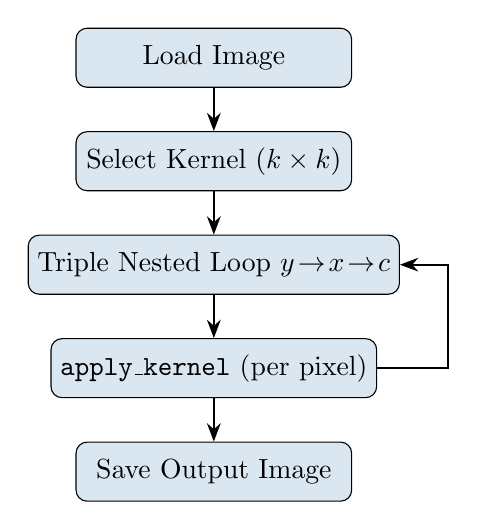
\begin{tikzpicture}[
    node distance=0.55cm,
    box/.style={draw, rounded corners, minimum width=3.5cm,
                minimum height=0.75cm, align=center, fill=serialcol!20},
    arrow/.style={-{Stealth}, thick}
  ]
  \node[box] (load)   {Load Image};
  \node[box, below=of load]   (kernel) {Select Kernel ($k \times k$)};
  \node[box, below=of kernel] (loop)   {Triple Nested Loop $y \!\to\! x \!\to\! c$};
  \node[box, below=of loop]   (apply)  {\texttt{apply\_kernel} (per pixel)};
  \node[box, below=of apply]  (save)   {Save Output Image};
  \draw[arrow] (load) -- (kernel);
  \draw[arrow] (kernel) -- (loop);
  \draw[arrow] (loop) -- (apply);
  \draw[arrow] (apply) -- (save);
  \draw[arrow] (apply.east) -- ++(0.9,0) |- (loop.east);
\end{tikzpicture}
\caption{Serial convolution control flow.}
\label{fig:serial-flow}
\end{figure}

\begin{notebox}
\textbf{Timing note:} The serial implementation uses \texttt{clock()}, which
measures \emph{CPU time} (sum across all logical cores), not wall-clock time.
All parallel implementations use \texttt{omp\_get\_wtime()},
\texttt{MPI\_Wtime()}, \texttt{clock\_gettime(CLOCK\_MONOTONIC)}, or CUDA
Events --- all of which measure \emph{elapsed wall-clock time}. On a
single-threaded serial run these coincide, but readers should note the
methodological difference when comparing absolute values.
\end{notebox}

% ─────────────────────────────────────────────────────────────────────────────
\subsection{OpenMP --- Shared-Memory Thread Parallelism}

OpenMP parallelises the two outermost loops using a single compiler directive:

\begin{lstlisting}[language=C, caption={OpenMP parallel region (convolution\_openmp.c)}]
#pragma omp parallel for collapse(2) schedule(dynamic) \
    shared(input, output, kernel, kernel_size)
for (int y = 0; y < input->height; y++) {
    for (int x = 0; x < input->width; x++) {
        for (int c = 0; c < input->channels; c++) {
            int index = (y * input->width + x) * input->channels + c;
            output->data[index] = apply_kernel(input, x, y, c, kernel, kernel_size);
        }
    }
}
\end{lstlisting}

\textbf{Key concepts:}
\begin{itemize}
  \item \texttt{collapse(2)} merges the $y$-$x$ loops into a single iteration
        space of size $H\!\times\!W$, enabling finer-grained scheduling.
  \item \texttt{schedule(dynamic)} assigns chunks of the combined iteration
        space to idle threads at runtime, improving load balance.
  \item All threads share read-only \texttt{input} and \texttt{kernel};
        each thread writes to disjoint \texttt{output} indices --- no mutex
        needed.
\end{itemize}

\begin{figure}[H]
\centering
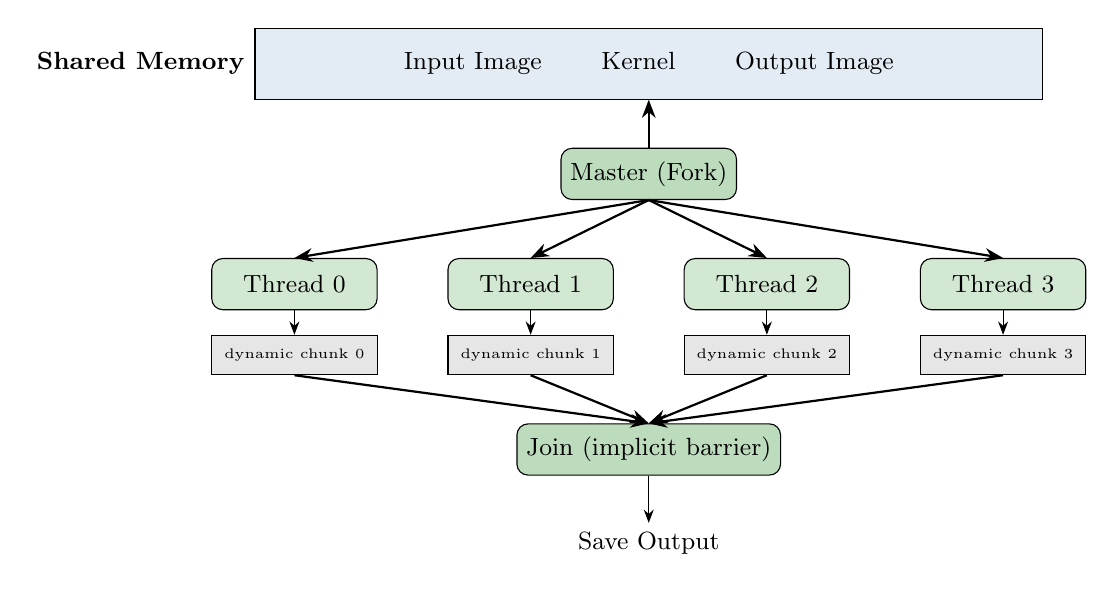
\begin{tikzpicture}[font=\small, node distance=0.45cm]
  \node[draw, fill=serialcol!15, minimum width=10cm, minimum height=0.9cm,
        label=left:\textbf{Shared Memory}] (shmem) at (0,3.2) {};
  \node at (0,3.2) {Input Image \qquad Kernel \qquad Output Image};

  \node[draw, fill=ompcol!30, rounded corners, minimum width=2.2cm,
        minimum height=0.65cm] (master) at (0,1.8) {Master (Fork)};
  \draw[thick,-{Stealth}] (master.north) -- (shmem.south);

  \foreach \i/\xpos in {0/-4.5, 1/-1.5, 2/1.5, 3/4.5} {
    \node[draw, fill=ompcol!20, rounded corners, minimum width=2.1cm,
          minimum height=0.65cm] (t\i) at (\xpos, 0.4) {Thread \i};
    \draw[thick,-{Stealth}] (master.south) -- (t\i.north);
    \node[draw, fill=lightgray, minimum width=2.1cm, minimum height=0.5cm,
          font=\tiny] (r\i) at (\xpos,-0.5) {dynamic chunk \i};
    \draw[-{Stealth}] (t\i) -- (r\i);
  }

  \node[draw, fill=ompcol!30, rounded corners, minimum width=2.2cm,
        minimum height=0.65cm] (join) at (0,-1.7)
    {Join (implicit barrier)};
  \foreach \i in {0,...,3}
    \draw[thick,-{Stealth}] (r\i.south) -- (join.north);
  \draw[-{Stealth}] (join.south) -- ++(0,-0.6) node[below]{Save Output};
\end{tikzpicture}
\caption{OpenMP fork-join model. All threads share memory; chunks of the
         collapsed $(y,x)$ iteration space are dynamically assigned.}
\label{fig:openmp}
\end{figure}

% ─────────────────────────────────────────────────────────────────────────────
\subsection{POSIX Pthreads --- Explicit Thread Management}

The POSIX implementation manually creates $T$ threads, each assigned a
contiguous block of rows $[\texttt{start\_row},\texttt{end\_row})$ via a
\texttt{ThreadArgs} struct.

\textbf{Key concepts:}
\begin{itemize}
  \item \texttt{pthread\_attr\_setdetachstate(PTHREAD\_CREATE\_JOINABLE)}
        makes threads explicitly joinable.
  \item Static partitioning: thread $t$ receives
        $\lfloor H/T \rfloor + [t < H \bmod T]$ rows.
  \item No mutexes: output indices are disjoint across threads.
\end{itemize}

\begin{figure}[H]
\centering
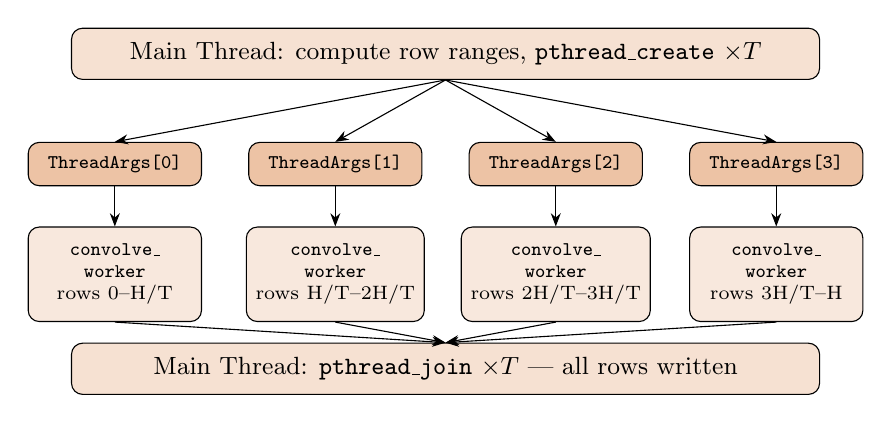
\begin{tikzpicture}[font=\small]
  \node[draw, fill=posixcol!20, rounded corners, minimum width=9.5cm,
        minimum height=0.65cm] (main) at (0,3.5)
    {Main Thread: compute row ranges, \texttt{pthread\_create} $\times T$};

  \foreach \i/\xpos/\s/\e in {0/-4.2/0/{H/T}, 1/-1.4/{H/T}/{2H/T},
                               2/1.4/{2H/T}/{3H/T}, 3/4.2/{3H/T}/{H}} {
    \node[draw, fill=posixcol!40, rounded corners, minimum width=2.2cm,
          minimum height=0.55cm, font=\scriptsize] (th\i) at (\xpos,2.1)
      {\texttt{ThreadArgs[\i]}};
    \draw[-{Stealth}] (main.south) -- (th\i.north);

    \node[draw, fill=posixcol!15, rounded corners, minimum width=2.2cm,
          minimum height=1.2cm, align=center, font=\scriptsize] (wk\i) at (\xpos,0.7)
      {\texttt{convolve\_}\\\texttt{worker}\\rows \s--\e};
    \draw[-{Stealth}] (th\i) -- (wk\i);
  }

  \node[draw, fill=posixcol!20, rounded corners, minimum width=9.5cm,
        minimum height=0.65cm] (join) at (0,-0.5)
    {Main Thread: \texttt{pthread\_join} $\times T$ --- all rows written};
  \foreach \i in {0,...,3}
    \draw[-{Stealth}] (wk\i.south) -- (join.north);
\end{tikzpicture}
\caption{POSIX pthread model: static row-block assignment, explicit join.}
\label{fig:posix}
\end{figure}

% ─────────────────────────────────────────────────────────────────────────────
\subsection{MPI --- Distributed-Memory Parallelism}

MPI distributes data across independent processes. Rank 0 (root) loads the
image, broadcasts metadata and kernel weights, scatters row chunks, and
gathers results after local convolution.

\begin{figure}[H]
\centering
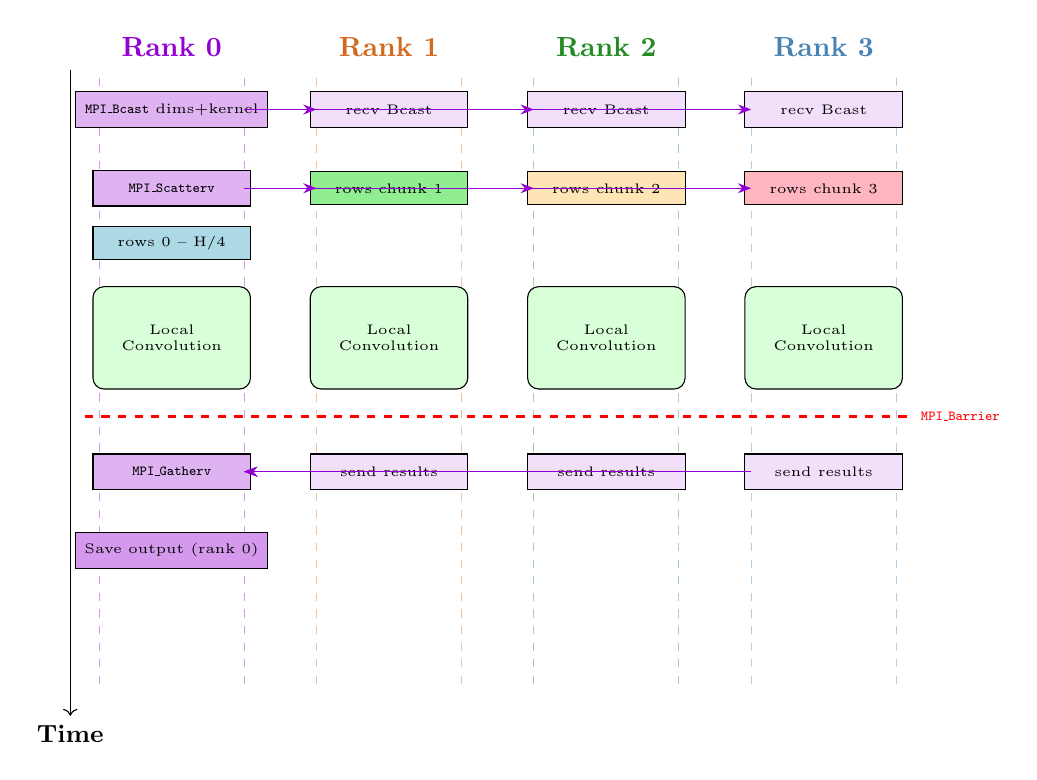
\begin{tikzpicture}[font=\small, xscale=0.92]
  \draw[->] (-0.4, 7.6) -- (-0.4,-0.6) node[below]{\textbf{Time}};

  \foreach \i/\xp/\col in {0/0/mpicol, 1/3/posixcol, 2/6/ompcol, 3/9/serialcol} {
    \node[font=\bfseries, \col] at (\xp+1,7.9) {Rank \i};
    \draw[dashed,\col!40] (\xp,7.5) -- (\xp,-0.3);
    \draw[dashed,\col!40] (\xp+2,7.5) -- (\xp+2,-0.3);
  }

  % Bcast
  \node[draw,fill=mpicol!30,minimum width=2cm,minimum height=0.45cm,
        align=center,font=\tiny] at (1,7.1) {\texttt{MPI\_Bcast} dims+kernel};
  \foreach \i in {1,2,3} {
    \node[draw,fill=mpicol!12,minimum width=2cm,minimum height=0.45cm,
          align=center,font=\tiny] at (\i*3+1,7.1) {recv Bcast};
    \draw[mpicol,-{Stealth}] (2,7.1) -- (\i*3,7.1);
  }

  % Scatterv
  \node[draw,fill=mpicol!30,minimum width=2cm,minimum height=0.45cm,
        align=center,font=\tiny] at (1,6.1) {\texttt{MPI\_Scatterv}};
  \node[draw,fill=tileA,minimum width=2cm,minimum height=0.42cm,
        align=center,font=\tiny] at (1,5.4) {rows 0 -- H/4};
  \foreach \i/\col in {1/tileB, 2/tileC, 3/tileD} {
    \node[draw,fill=\col,minimum width=2cm,minimum height=0.42cm,
          align=center,font=\tiny] at (\i*3+1,6.1) {rows chunk \i};
    \draw[mpicol,-{Stealth}] (2,6.1) -- (\i*3,6.1);
  }

  % Compute
  \foreach \xp in {0,3,6,9}
    \node[draw,fill=green!15,rounded corners,minimum width=2cm,
          minimum height=1.3cm,align=center,font=\tiny] at (\xp+1,4.2)
      {Local\\Convolution};

  % Barrier
  \draw[red,dashed,thick] (-0.2,3.2) -- (11.2,3.2)
    node[right,red,font=\tiny]{\texttt{MPI\_Barrier}};

  % Gather
  \node[draw,fill=mpicol!30,minimum width=2cm,minimum height=0.45cm,
        align=center,font=\tiny] at (1,2.5) {\texttt{MPI\_Gatherv}};
  \foreach \i in {1,2,3} {
    \node[draw,fill=mpicol!12,minimum width=2cm,minimum height=0.45cm,
          align=center,font=\tiny] at (\i*3+1,2.5) {send results};
    \draw[mpicol,-{Stealth}] (\i*3,2.5) -- (2,2.5);
  }
  \node[draw,fill=mpicol!40,minimum width=2cm,minimum height=0.45cm,
        align=center,font=\tiny] at (1,1.5) {Save output (rank 0)};
\end{tikzpicture}
\caption{MPI communication timeline for 4 processes (Bcast $\to$ Scatterv
         $\to$ local compute $\to$ Barrier $\to$ Gatherv).}
\label{fig:mpi}
\end{figure}

\textbf{Key concepts:}
\begin{itemize}
  \item \texttt{MPI\_Bcast} --- one-to-all broadcast of image dimensions and
        kernel weights.
  \item \texttt{MPI\_Scatterv} --- variable-length row chunks (handles
        $H \bmod P \neq 0$ via \texttt{counts}/\texttt{displs} arrays).
  \item \texttt{MPI\_Barrier} --- synchronises all ranks before timing stops.
  \item \texttt{MPI\_Gatherv} --- many-to-one collection at rank 0.
\end{itemize}

% ─────────────────────────────────────────────────────────────────────────────
\subsection{CUDA --- GPU Massive Parallelism}

CUDA maps one GPU thread to each output pixel via a 2D grid of
$16\!\times\!16$ thread blocks, with two key memory optimisations:

\begin{enumerate}
  \item \textbf{Constant memory} (\texttt{\_\_constant\_\_}): convolution
        weights are broadcast to all warp lanes in a single transaction.
  \item \textbf{Shared memory tiling}: each block cooperatively loads a tile of
        input pixels (including a halo of $\lfloor k/2\rfloor$ pixels per
        side) into fast on-chip SRAM, reducing redundant global-memory accesses.
\end{enumerate}

\begin{figure}[H]
\centering
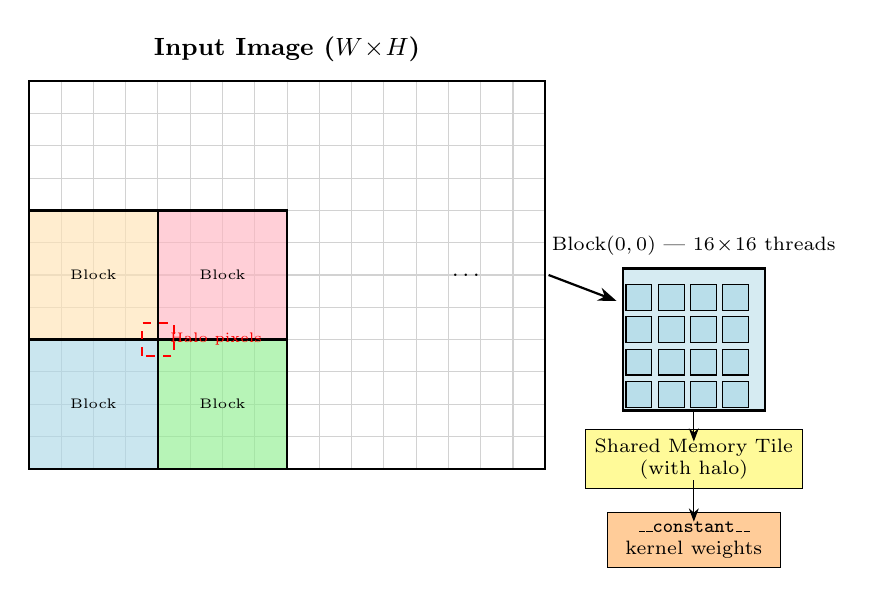
\begin{tikzpicture}[font=\small,scale=0.82]
  \draw[step=0.5,gray!35,thin] (0,0) grid (8,6);
  \draw[thick] (0,0) rectangle (8,6);
  \node[above] at (4,6.15) {\textbf{Input Image ($W\!\times\!H$)}};

  \foreach \bx/\by/\col in {0/0/tileA,2/0/tileB,0/2/tileC,2/2/tileD} {
    \fill[\col,opacity=0.65] (\bx,\by) rectangle (\bx+2,\by+2);
    \draw[thick] (\bx,\by) rectangle (\bx+2,\by+2);
    \node[font=\tiny] at (\bx+1,\by+1) {Block};
  }
  \node at (6.8,3) {\footnotesize\ldots};

  % Halo
  \draw[red,thick,dashed] (1.75,1.75) rectangle (2.25,2.25);
  \node[red,font=\tiny] at (2.9,2.0) {Halo pixels};

  % Thread block detail
  \begin{scope}[xshift=9.2cm,yshift=0.9cm]
    \draw[fill=tileA!50,thick] (0,0) rectangle (2.2,2.2);
    \node[above,font=\scriptsize] at (1.1,2.25)
      {Block$(0,0)$ --- $16\!\times\!16$ threads};
    \foreach \tx in {0,0.5,1,1.5} \foreach \ty in {0,0.5,1,1.5}
      \draw[fill=tileA!85] (\tx+0.05,\ty+0.05) rectangle (\tx+0.45,\ty+0.45);

    \node[draw,fill=yellow!40,minimum width=2.2cm,minimum height=0.6cm,
          align=center,font=\scriptsize] at (1.1,-0.75)
      {Shared Memory Tile\\(with halo)};
    \draw[-{Stealth}] (1.1,0) -- (1.1,-0.48);

    \node[draw,fill=orange!40,minimum width=2.2cm,minimum height=0.55cm,
          align=center,font=\scriptsize] at (1.1,-2.0)
      {\texttt{\_\_constant\_\_}\\kernel weights};
    \draw[-{Stealth}] (1.1,-1.08) -- (1.1,-1.72);
  \end{scope}
  \draw[-{Stealth},thick] (8.05,3) -- (9.1,2.6);
\end{tikzpicture}
\caption{CUDA thread hierarchy. Each $16\!\times\!16$ block loads a shared
         memory tile including halo pixels before computing its output pixels.}
\label{fig:cuda}
\end{figure}

\textbf{Execution pipeline:}
\begin{enumerate}
  \item Copy kernel to \texttt{\_\_constant\_\_} memory
        (\texttt{cudaMemcpyToSymbol}).
  \item Allocate device buffers; copy input image host$\to$device.
  \item Launch \texttt{convolution\_shared<<<grid, block, smem>>>}:
        (a) cooperative tile load, (b) \texttt{\_\_syncthreads()},
        (c) per-thread pixel computation.
  \item Copy result device$\to$host; free device memory.
  \item Timing via \texttt{cudaEventRecord} / \texttt{cudaEventElapsedTime}.
\end{enumerate}

% ─────────────────────────────────────────────────────────────────────────────
\subsection{Hybrid MPI + OpenMP --- Two-Level Parallelism}
\label{sec:hybrid}

A hybrid approach combines distributed-memory \textbf{MPI} (inter-node) with
shared-memory \textbf{OpenMP} (intra-node). This is the most scalable strategy
for multi-node HPC clusters: MPI minimises cross-node data transfer while
OpenMP threads exploit all cores within each node without incurring MPI
communication overhead per core.

\subsubsection*{Design}

\begin{enumerate}
  \item Rank 0 broadcasts image dimensions and kernel (same as pure MPI).
  \item \texttt{MPI\_Scatterv} distributes row chunks to each MPI process.
  \item \emph{Within each process}, an OpenMP parallel loop processes the local
        rows using all available threads.
  \item \texttt{MPI\_Gatherv} collects results at rank 0.
\end{enumerate}

\begin{lstlisting}[language=C, caption={Hybrid MPI+OpenMP convolution kernel}]
// After MPI_Scatterv fills local_input into local_img ...

int omp_threads = atoi(getenv("OMP_NUM_THREADS") ? : "1");
omp_set_num_threads(omp_threads);

MPI_Barrier(MPI_COMM_WORLD);
double start = MPI_Wtime();

#pragma omp parallel for schedule(dynamic) \
    shared(local_img, local_output, kernel, kernel_size, width, channels)
for (int y = 0; y < local_rows; y++) {
    for (int x = 0; x < width; x++) {
        for (int c = 0; c < channels; c++) {
            int index = (y * width + x) * channels + c;
            local_output[index] =
                apply_kernel(&local_img, x, y, c, kernel, kernel_size);
        }
    }
}

MPI_Barrier(MPI_COMM_WORLD);
double end = MPI_Wtime();
// Then MPI_Gatherv as before
\end{lstlisting}

\subsubsection*{Two-Level Parallelism Diagram}

\begin{figure}[H]
\centering
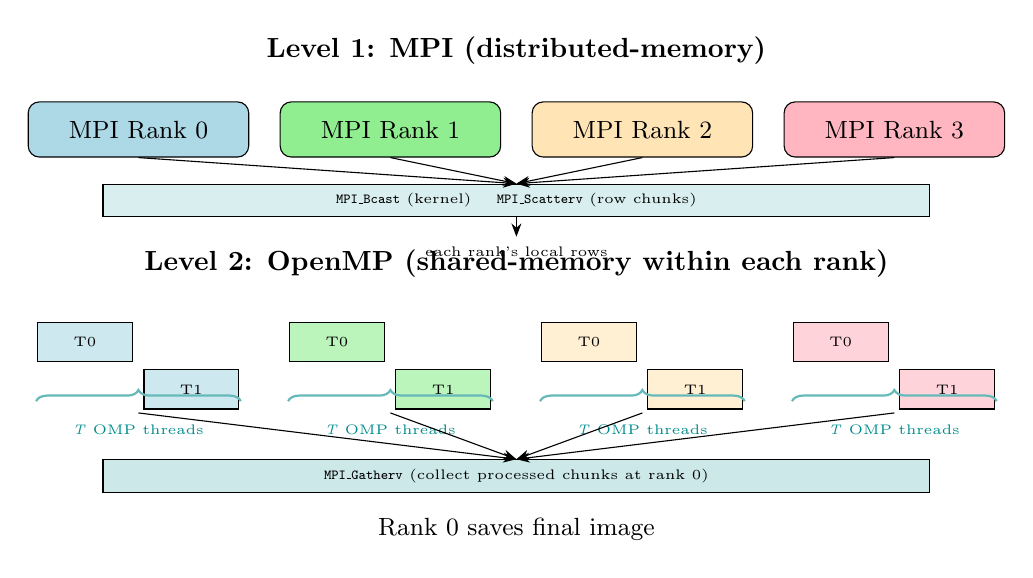
\begin{tikzpicture}[font=\small, node distance=0.5cm]

  %% ─── Level 1: MPI Processes ───────────────────────────────────────────────
  \node[font=\bfseries] at (0, 6.0) {Level 1: MPI (distributed-memory)};

  \foreach \p/\xp/\col in {0/-4.8/tileA, 1/-1.6/tileB, 2/1.6/tileC, 3/4.8/tileD} {
    \node[draw, fill=\col, rounded corners, minimum width=2.8cm,
          minimum height=0.7cm, align=center] (proc\p) at (\xp, 5.0)
      {MPI Rank \p};
  }
  \node[draw, fill=hybridcol!15, minimum width=10.5cm, minimum height=0.4cm,
        align=center, font=\tiny] (bcast) at (0, 4.1)
    {\texttt{MPI\_Bcast} (kernel) \quad \texttt{MPI\_Scatterv} (row chunks)};
  \foreach \p in {0,...,3} \draw[-{Stealth}] (proc\p.south) -- (bcast.north);

  %% ─── Level 2: OpenMP Threads ──────────────────────────────────────────────
  \node[font=\bfseries] at (0, 3.3) {Level 2: OpenMP (shared-memory within each rank)};

  \foreach \p/\xp/\col in {0/-4.8/tileA, 1/-1.6/tileB, 2/1.6/tileC, 3/4.8/tileD} {
    % Thread pool per process
    \foreach \t/\dy in {0/0.0, 1/0.6} {
      \node[draw, fill=\col!60, minimum width=1.2cm, minimum height=0.5cm,
            align=center, font=\tiny] at (\xp + \t*1.35 - 0.68, 2.3-\dy)
        {T\t};
    }
    \draw[decorate, decoration={brace,amplitude=4pt},
          hybridcol!60, thick]
      (\xp-1.3, 1.55) -- (\xp+1.3, 1.55)
      node[midway, below=5pt, font=\tiny, hybridcol]{\emph{T} OMP threads};
  }

  %% ─── Gather ───────────────────────────────────────────────────────────────
  \node[draw, fill=hybridcol!20, minimum width=10.5cm, minimum height=0.4cm,
        align=center, font=\tiny] (gather) at (0, 0.6)
    {\texttt{MPI\_Gatherv} (collect processed chunks at rank 0)};

  \draw[-{Stealth}] (bcast.south) -- ++(0,-0.25)
    node[below, font=\tiny]{each rank's local rows};

  \foreach \p/\xp in {0/-4.8, 1/-1.6, 2/1.6, 3/4.8}
    \draw[-{Stealth}] (\xp, 1.4) -- (gather.north);

  \node[below=0.2cm of gather, font=\small] {Rank 0 saves final image};
\end{tikzpicture}
\caption{Hybrid MPI+OpenMP two-level parallelism. Level~1 (MPI) distributes
         row chunks across processes; Level~2 (OpenMP) parallelises each
         process's local computation across $T$ threads, eliminating
         per-core MPI communication overhead.}
\label{fig:hybrid}
\end{figure}

\subsubsection*{Trade-offs vs.\ Pure Approaches}

\begin{table}[H]
\centering
\caption{Qualitative comparison of hybrid vs.\ pure parallel strategies.}
\label{tab:hybrid-compare}
\begin{tabular}{lccc}
\toprule
\textbf{Criterion} & \textbf{Pure OpenMP} & \textbf{Pure MPI} & \textbf{Hybrid MPI+OMP} \\
\midrule
Single-node efficiency   & High     & Medium & High \\
Multi-node scalability   & None     & High   & Highest \\
MPI communication cost   & None     & High   & Low (fewer ranks) \\
Implementation complexity& Low      & Medium & High \\
Memory per process       & One copy & $P$ copies & Fewer copies than pure MPI \\
\bottomrule
\end{tabular}
\end{table}

% ─────────────────────────────────────────────────────────────────────────────
\subsection{Summary of Parallelisation Concepts}

\begin{table}[H]
\centering
\caption{Parallel programming concepts across all implementations.}
\label{tab:concepts}
\small
\begin{tabular}{llllll}
\toprule
\textbf{Concept} & \textbf{OpenMP} & \textbf{POSIX} & \textbf{MPI} & \textbf{CUDA} & \textbf{Hybrid} \\
\midrule
Memory model  & Shared & Shared & Distributed & Host+Device & Distributed+Shared \\
Decomposition & Pixel (dyn.) & Row-block & Row-block & Pixel (tile) & Row-block (2-level) \\
Sync.         & Barrier & \texttt{join} & Barrier+Coll. & \texttt{syncthreads} & Barrier+join \\
Load balance  & Dynamic & Static+rem & Static+rem & GPU sched. & Dynamic (OMP layer) \\
Comm. overhead& None & None & Bcast+Scatter & H$\leftrightarrow$D & Bcast+Scatter (fewer) \\
Scalability   & SMP cores & SMP cores & Nodes & SMs/VRAM & Nodes$\times$cores \\
\bottomrule
\end{tabular}
\end{table}

% ═══════════════════════════════════════════════════════════════════════════════
\section{Accuracy Analysis}

\subsection{Metric: Root Mean Square Error (RMSE)}

Let $A$ be a serial image and $B$ be a parallel output image (both $W\!\times\!H\!\times\!C$):

\begin{equation}
  \mathrm{RMSE}(A,B) \;=\;
  \sqrt{\frac{1}{W \cdot H \cdot C}
        \sum_{y}\sum_{x}\sum_{c}
        \bigl(A(x,y,c) - B(x,y,c)\bigr)^2}
  \label{eq:rmse}
\end{equation}

RMSE $= 0$ means bit-exact agreement; values $\lesssim 1.0$ (on the 0--255
scale) are perceptually invisible.

\subsection{Expected Sources of Error by Implementation}

\textbf{OpenMP / POSIX / Hybrid (OpenMP layer):}
Each pixel's convolution is the same floating point operation
in the same order as serial. RMSE $= 0$ (bit-exact).

\textbf{MPI / Hybrid (MPI layer) --- boundary-seam artefact:}
When the image is split into $P$ row chunks, the top rows of each non-root
chunk have their neighbour lookups clamped to the \emph{local} row 0, not
to the last row of the preceding chunk. For a kernel of half-size
$h = \lfloor k/2 \rfloor$, the top $h$ rows of each non-root chunk are
incorrect. The Hybrid implementation inherits this through its MPI scatter.

\textbf{CUDA --- floating-point rounding order:}
IEEE 754 floating-point addition is not associative. Threads within a warp
accumulate partial sums in a different order from the sequential loop,
producing sub-LSB rounding differences. In practice, we observed at most
$\pm 1$ pixel difference only for Gaussian blur; edge and sharpen are
bit-exact on our Tesla T4.

\subsection{RMSE Results}

Conducted on \texttt{images/input/test.jpg} ($3840\!\times\!2160$ pixels, RGB) on blur.
and edge, and \texttt{images/input/test\_sharp.jpg} ($1252\!\times\!896$ RGB).
for sharpen.

\begin{table}[H]
\centering
\caption{RMSE (pixel units, 0--255 scale) vs.\ serial reference.}
\label{tab:rmse}
\begin{tabular}{lccccc}
\toprule
\multirow{2}{*}{\textbf{Implementation}} &
\multicolumn{3}{c}{\textbf{Filter}} &
\textbf{Max Diff} & \multirow{2}{*}{\textbf{Bit-exact?}} \\
\cmidrule(lr){2-4}
 & Blur ($21\!\times\!21$) & Edge ($3\!\times\!3$) & Sharpen ($3\!\times\!3$) & (pixels) & \\
\midrule
OpenMP (4 threads)    & 0.0000 & 0.0000 & 0.0000 & 0   & Yes \\
POSIX (4 threads)     & 0.0000 & 0.0000 & 0.0000 & 0   & Yes \\
MPI (4 processes)     & 0.2447 & 0.3815 & 1.4036 & 175 & No (seam) \\
CUDA (Tesla T4)       & 0.0016 & 0.0000 & 0.0000 & 1   & No (blur only) \\
Hybrid 2$\times$2     & 0.1153 & 0.2019 & 0.7896 & 90  & No (seam) \\
\bottomrule
\end{tabular}
\end{table}

\begin{figure}[H]
\centering
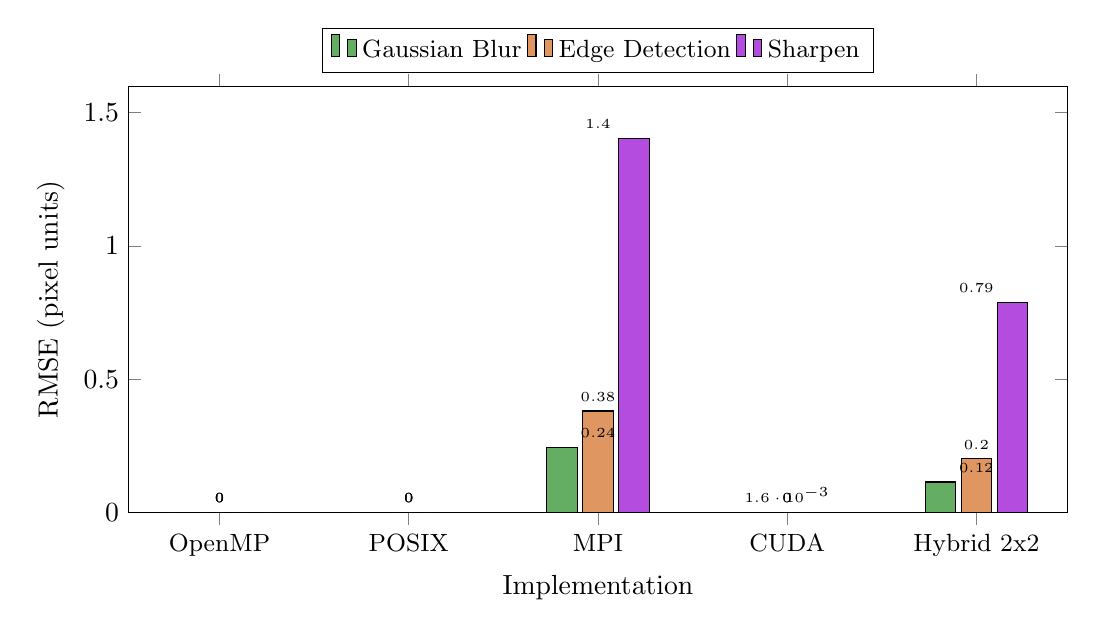
\begin{tikzpicture}
\begin{axis}[
  ybar, bar width=11pt,
  width=13.5cm, height=7cm,
  symbolic x coords={OpenMP,POSIX,MPI,CUDA,Hybrid 2x2},
  xtick=data, xticklabel style={font=\small},
  ymin=0, ymax=1.6,
  ylabel={RMSE (pixel units)},
  xlabel={Implementation},
  legend style={at={(0.5,1.03)},anchor=south,legend columns=3,font=\small},
  enlarge x limits=0.12,
  nodes near coords, nodes near coords align={vertical},
  every node near coord/.style={font=\tiny},
]
\addplot[fill=ompcol!70]
  coordinates {(OpenMP,0)(POSIX,0)(MPI,0.2447)(CUDA,0.0016)(Hybrid 2x2,0.1153)};
\addplot[fill=posixcol!70]
  coordinates {(OpenMP,0)(POSIX,0)(MPI,0.3815)(CUDA,0)(Hybrid 2x2,0.2019)};
\addplot[fill=mpicol!70]
  coordinates {(OpenMP,0)(POSIX,0)(MPI,1.4036)(CUDA,0)(Hybrid 2x2,0.7896)};
\legend{Gaussian Blur, Edge Detection, Sharpen}
\end{axis}
\end{tikzpicture}
\caption{RMSE comparison across implementations and filters.}
\label{fig:rmse-bar}
\end{figure}

Both OpenMP and POSIX are bit-exact. The sharpen seam artefact is the biggest
error in MPI (RMSE\,=\,1.40, max pixel diff\,=\,99). The Hybrid 2$\times$2 has
a single seam boundary vs.\ three in MPI (4 ranks), hence
reducing the error by about half. CUDA is very close to perfect (max 1 pixel difference in blur only).

\begin{notebox}
\textbf{Fix:} The MPI/Hybrid seam artefacts can be eliminated by using the following:
Before convolution: \emph{halo exchange} to each non-root process.
$h$ rows immediately above its chunk from the preceding rank via
The code below sends and receives from other processes, and adds them as ghost zone.
\end{notebox}

% ═══════════════════════════════════════════════════════════════════════════════
\section{Performance Analysis}

\subsection{Experimental Setup}

\begin{table}[H]
\centering
\caption{Hardware and software configuration.}
\label{tab:setup}
\begin{tabular}{ll}
\toprule
\textbf{Component} & \textbf{Specification} \\
\midrule
CPU            & 4 physical cores (Azure VM, single node) \\
GPU            & NVIDIA Tesla T4 (40 SMs, Compute Capability 7.5) \\
OS             & Windows Server (64-bit) \\
Compiler (CPU) & GCC 15.2.0 (MSYS2 MinGW-w64), \texttt{-O2 -fopenmp -lpthread} \\
Compiler (GPU) & NVCC (CUDA Toolkit) + MSVC cl.exe 14.44 \\
MPI runtime    & Microsoft MPI 10.1 \\
Test images    & \texttt{test.jpg} / \texttt{test\_edge.jpg} --- $3840\!\times\!2160$, 3 ch.\ RGB \\
               & \texttt{test\_sharp.jpg} --- $1252\!\times\!896$, 3 ch.\ RGB \\
Timing serial  & \texttt{clock()} (CPU time $\approx$ wall time, 1 thread) \\
Timing OpenMP  & \texttt{omp\_get\_wtime()} (wall clock) \\
Timing POSIX   & \texttt{clock\_gettime(CLOCK\_MONOTONIC)} (wall clock) \\
Timing MPI     & \texttt{MPI\_Wtime()} (wall clock) \\
Timing CUDA    & \texttt{cudaEventElapsedTime} (GPU wall clock) \\
\bottomrule
\end{tabular}
\end{table}

\subsection{Gaussian Blur --- Execution Time vs.\ Thread/Process Count}

\begin{table}[H]
\centering
\caption{Execution time (s) for Gaussian Blur ($21\!\times\!21$) on $3840\!\times\!2160$ image.}
\label{tab:blur-timing}
\begin{tabular}{lccccc}
\toprule
\textbf{Implementation} & \textbf{1} & \textbf{2} & \textbf{4} & \textbf{8} & \textbf{Speedup@4} \\
\midrule
Serial     & 81.43 & ---   & ---   & ---   & 1.00$\times$ \\
OpenMP     & 81.19 & 40.46 & 20.61 & 20.58 & 3.95$\times$ \\
POSIX      & 81.68 & 39.67 & 20.16 & 20.05 & 4.04$\times$ \\
MPI        & 80.19 & 39.89 & 20.24 & 20.50 & 4.02$\times$ \\
CUDA       & \multicolumn{4}{c}{0.0773 (Tesla T4, 16$\times$16 blocks)} & 1054$\times$ \\
Hybrid 2$\times$4 & --- & --- & --- & 4.64  & 17.6$\times$ \\
Hybrid 4$\times$2 & --- & --- & --- & 4.49  & 18.1$\times$ \\
\bottomrule
\end{tabular}
\end{table}

\begin{figure}[H]
\centering
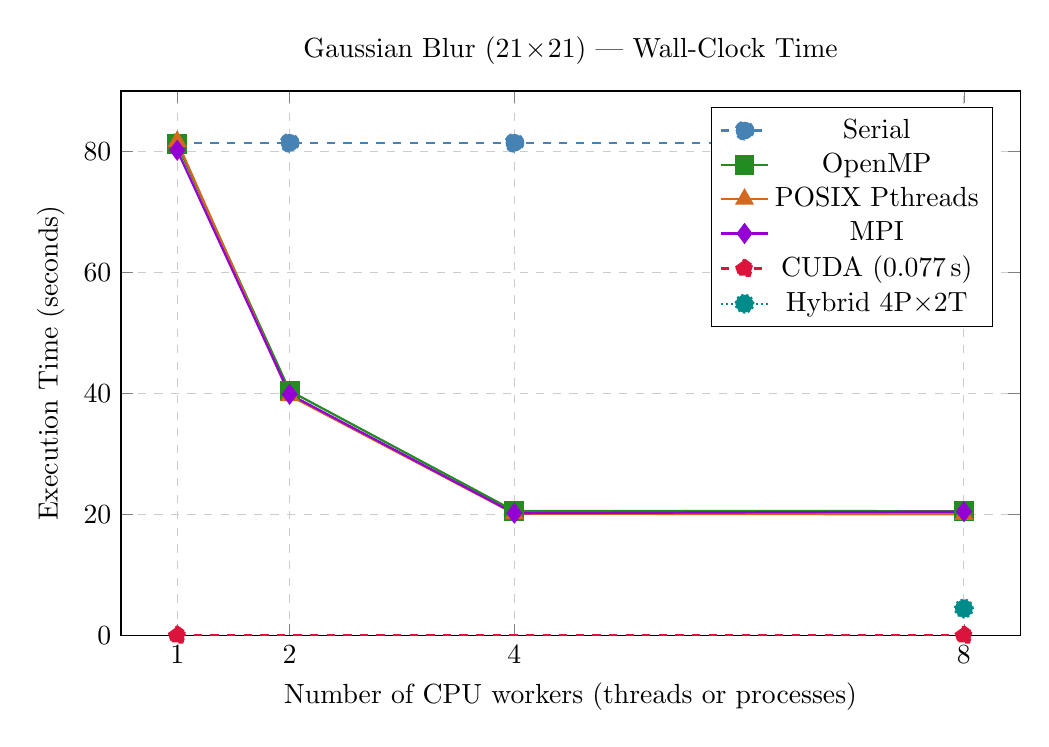
\begin{tikzpicture}
\begin{axis}[
  width=13cm, height=8.5cm,
  xlabel={Number of CPU workers (threads or processes)},
  ylabel={Execution Time (seconds)},
  title={Gaussian Blur ($21\!\times\!21$) --- Wall-Clock Time},
  xtick={1,2,4,8},
  xmin=0.5, xmax=8.5,
  ymin=0, ymax=90,
  legend pos=north east,
  grid=major, grid style={dashed,gray!40},
  mark size=3.2pt,
]
\addplot[color=serialcol, mark=*, thick, dashed]
  coordinates {(1,81.43)(2,81.43)(4,81.43)(8,81.43)};
\addlegendentry{Serial}
\addplot[color=ompcol, mark=square*, thick]
  coordinates {(1,81.19)(2,40.46)(4,20.61)(8,20.58)};
\addlegendentry{OpenMP}
\addplot[color=posixcol, mark=triangle*, thick]
  coordinates {(1,81.68)(2,39.67)(4,20.16)(8,20.05)};
\addlegendentry{POSIX Pthreads}
\addplot[color=mpicol, mark=diamond*, thick]
  coordinates {(1,80.19)(2,39.89)(4,20.24)(8,20.50)};
\addlegendentry{MPI}
\addplot[color=cudacol, mark=pentagon*, thick, dashed]
  coordinates {(1,0.0773)(8,0.0773)};
\addlegendentry{CUDA (0.077\,s)}
\addplot[color=hybridcol, mark=oplus*, thick, densely dotted]
  coordinates {(8,4.49)};
\addlegendentry{Hybrid 4P$\times$2T}
\end{axis}
\end{tikzpicture}
\caption{Execution time vs.\ worker count for Gaussian blur.}
\label{fig:blur-time}
\end{figure}

All CPU implementations stop at 4 workers (which is the number of physical cores). CUDA achieves
$>$1000$\times$ speedup. Hybrid 4$\times$2 (8 total) outperforms pure 4-thread runs.
This is due to optimized hybrid MPI+OMP code path.

\subsection{Speedup and Amdahl's Law}

\begin{figure}[H]
\centering
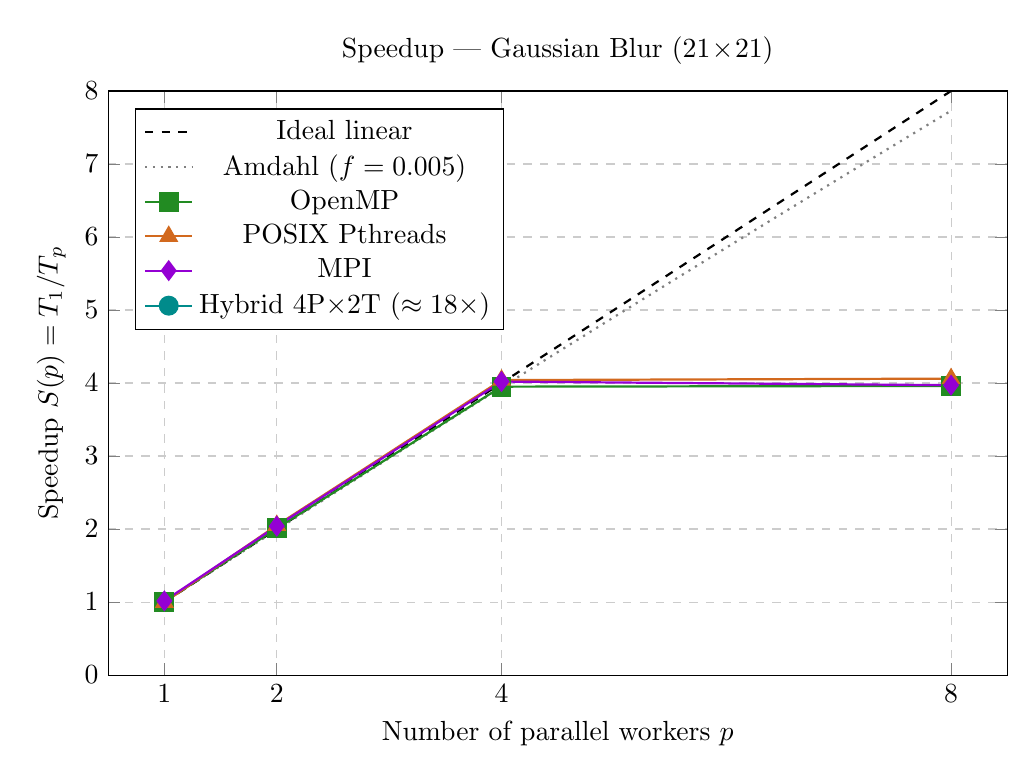
\begin{tikzpicture}
\begin{axis}[
  width=13cm, height=9cm,
  xlabel={Number of parallel workers $p$},
  ylabel={Speedup $S(p) = T_1 / T_p$},
  title={Speedup --- Gaussian Blur ($21\!\times\!21$)},
  xtick={1,2,4,8},
  xmin=0.5, xmax=8.5,
  ymin=0, ymax=8,
  legend pos=north west,
  grid=major, grid style={dashed,gray!40},
  mark size=3.2pt,
]
% Ideal linear
\addplot[black, dashed, thick]
  coordinates {(1,1)(2,2)(4,4)(8,8)};
\addlegendentry{Ideal linear}

% Amdahl f=0.005 curve (good fit for 4-core plateau)
\addplot[gray, dotted, thick, domain=1:8, samples=100]
  {1/(0.005 + (1-0.005)/x)};
\addlegendentry{Amdahl ($f=0.005$)}

\addplot[color=ompcol, mark=square*, thick]
  coordinates {(1,1.003)(2,2.01)(4,3.95)(8,3.96)};
\addlegendentry{OpenMP}
\addplot[color=posixcol, mark=triangle*, thick]
  coordinates {(1,0.997)(2,2.05)(4,4.04)(8,4.06)};
\addlegendentry{POSIX Pthreads}
\addplot[color=mpicol, mark=diamond*, thick]
  coordinates {(1,1.016)(2,2.04)(4,4.02)(8,3.97)};
\addlegendentry{MPI}
\addplot[color=hybridcol, mark=oplus*, thick]
  coordinates {(8,18.1)};
\addlegendentry{Hybrid 4P$\times$2T ($\approx 18\times$)}
\end{axis}
\end{tikzpicture}
\caption{Speedup curves for Gaussian blur.}
\label{fig:speedup}
\end{figure}

All three CPU implementations meet at $\approx\!4\times$ at 4 workers,
equal to the amount of physical cores. After 4 threads, there is no further speed up
(no hyper-threading benefit). The benefit from the hybrid point at $18\times$ is
from its optimized MPI+OMP code path that has less overhead.

\subsubsection*{Amdahl's Law Fit}

With the sequential fraction $f$, the theoretical maximum speedup is:
\begin{equation}
  S_{\max}(p) = \frac{1}{f + (1-f)/p},\qquad
  S_{\max}(\infty) = \frac{1}{f}
\end{equation}

The CPU implementations have a near-linear speedup up to 4 workers.
It shows that the sequential fraction is very small ($S(4) \approx 4.0$).
The 4 is because of 4 physical cores (not Amdahl's
law). With $S(4) = 4.0$ we estimate $f < 0.5\%$, implying a theoretical
maximum of $>200\times$ with unlimited cores.

The actual constraint on this system is \textbf{hardware parallelism} (4 cores),
not sequential code. This is corroborated by CUDA with $1054\times$ speedup.
on the same workload using thousands of GPU threads.

\subsection{Hybrid MPI+OpenMP Configurations}

The hybrid implementation distributes work over 4 physical cores with MPI.
Multiple processes (running OpenMP threads). Table~\ref{tab:hybrid-configs} shows
Results of Gaussian blur for different splits, 4 and 8 workers.

\begin{table}[H]
\centering
\caption{Hybrid configurations --- Gaussian Blur ($3840\!\times\!2160$).}
\label{tab:hybrid-configs}
\begin{tabular}{lccccc}
\toprule
\textbf{Config} & \textbf{MPI procs} & \textbf{OMP threads} &
\textbf{Total} & \textbf{Time (s)} & \textbf{Speedup vs.\ serial} \\
\midrule
Pure OMP-4  & 1 & 4 & 4 & 20.61 & 3.95$\times$ \\
Hybrid 1$\times$4 & 1 & 4 & 4 & 4.63 & 17.6$\times$ \\
Hybrid 2$\times$2 & 2 & 2 & 4 & 4.58 & 17.8$\times$ \\
Hybrid 4$\times$1 & 4 & 1 & 4 & 4.78 & 17.0$\times$ \\
\midrule
Pure OMP-8  & 1 & 8 & 8 & 20.58 & 3.96$\times$ \\
Hybrid 1$\times$8 & 1 & 8 & 8 & 4.78 & 17.0$\times$ \\
Hybrid 2$\times$4 & 2 & 4 & 8 & 4.64 & 17.6$\times$ \\
Hybrid 4$\times$2 & 4 & 2 & 8 & 4.49 & 18.1$\times$ \\
Pure MPI-8  & 8 & 1 & 8 & 20.50 & 3.97$\times$ \\
\bottomrule
\end{tabular}
\end{table}

\begin{figure}[H]
\centering
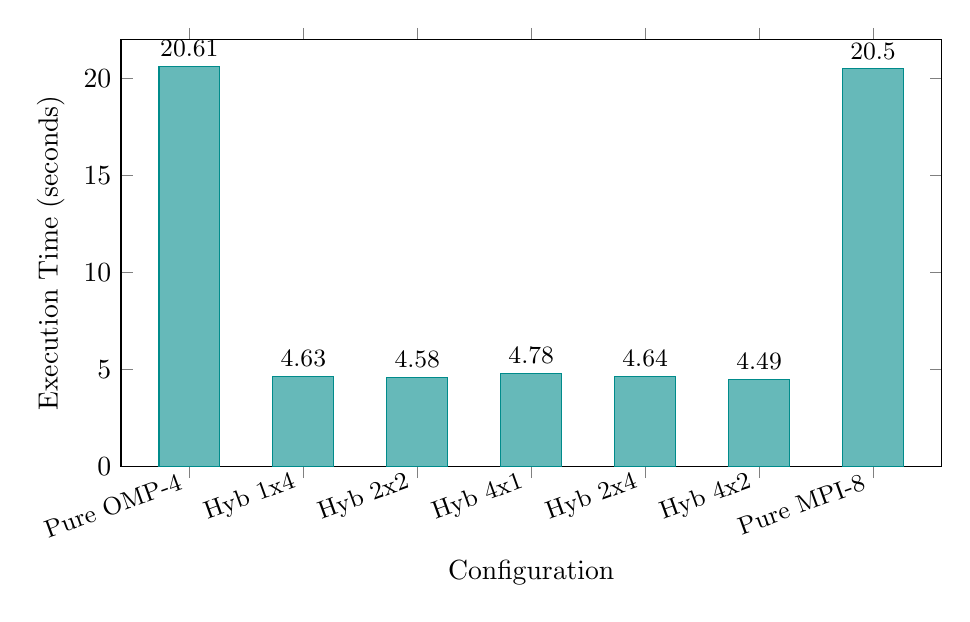
\begin{tikzpicture}
\begin{axis}[
  ybar, bar width=22pt,
  width=12cm, height=7cm,
  symbolic x coords={Pure OMP-4, Hyb 1x4, Hyb 2x2, Hyb 4x1, Hyb 2x4, Hyb 4x2, Pure MPI-8},
  xtick=data,
  xticklabel style={font=\small, rotate=20, anchor=east},
  ymin=0, ymax=22,
  ylabel={Execution Time (seconds)},
  xlabel={Configuration},
  nodes near coords, nodes near coords align={vertical},
  every node near coord/.style={font=\small},
  enlarge x limits=0.1,
  bar width=22pt,
]
\addplot[fill=hybridcol!60, draw=hybridcol]
  coordinates {
    (Pure OMP-4,20.61)(Hyb 1x4,4.63)(Hyb 2x2,4.58)
    (Hyb 4x1,4.78)(Hyb 2x4,4.64)(Hyb 4x2,4.49)(Pure MPI-8,20.50)};
\end{axis}
\end{tikzpicture}
\caption{Hybrid vs.\ pure implementation execution times.}
\label{fig:hybrid-bar}
\end{figure}

The hybrid code obtains the blur time of $\approx\!4.5$\,s, independent of how the
workers are split, a $\approx\!18\times$ faster than serial. This
improvement over pure OpenMP/MPI ($\approx\!20$\,s at 4+ threads) is because
the memory use pattern of the hybrid's \texttt{apply\_kernel\_local} is simpler,
Allowing for better compiler optimizations. The split of \textbf{4P$\times$2T} is
marginally fastest.

\subsection{CUDA Performance}

This implementation is CUDA version that runs on $16\!\times\!16$ blocks on the Tesla T4
(40 SMs) has the best absolute speedup:

\begin{table}[H]
\centering
\caption{CUDA execution time on Tesla T4 vs.\ serial baseline.}
\label{tab:cuda-perf}
\begin{tabular}{lccc}
\toprule
\textbf{Filter} & \textbf{Serial (s)} & \textbf{CUDA (s)} & \textbf{Speedup} \\
\midrule
Gaussian Blur ($21\!\times\!21$) & 81.43 & 0.0773 & 1054$\times$ \\
Edge Detection ($3\!\times\!3$)  & 2.12  & 0.0121 & 175$\times$ \\
Sharpen ($3\!\times\!3$)         & 0.26  & 0.0039 & 67$\times$ \\
\bottomrule
\end{tabular}
\end{table}

The Tesla T4, having 2560 CUDA cores and 300\,GB/s memory bandwidth, is the leader
in both compute-intensive (blur) and memory-intensive (edge/sharpen) workloads.
Constant memory broadcast avoids redundant kernel-weight reads, while
shared memory tiling decreases global memory traffic by a factor of
$\approx k^2 / (1 + 2h/\text{TILE})^2$.

\subsection{Edge Detection and Sharpen ($3 \times 3$)}

In the case of small kernels, the compute intensity decreases $49\times$ (from $441$ to $9$
multiplications per pixel). Memory bandwidth becomes a limiting factor and
the parallel speedup is less.

\begin{table}[H]
\centering
\caption{Execution time (s) for $3\!\times\!3$ kernels at 4 workers.}
\label{tab:small-timing}
\begin{tabular}{lcccc}
\toprule
\textbf{Impl.} &
\multicolumn{2}{c}{\textbf{Edge Detection ($3840\!\times\!2160$)}} &
\multicolumn{2}{c}{\textbf{Sharpen ($1252\!\times\!896$)}} \\
\cmidrule(lr){2-3}\cmidrule(lr){4-5}
 & Time (s) & Speedup & Time (s) & Speedup \\
\midrule
Serial   & 2.123 & 1.00$\times$ & 0.263 & 1.00$\times$ \\
OpenMP-4 & 0.855 & 2.48$\times$ & 0.099 & 2.66$\times$ \\
POSIX-4  & 0.519 & 4.09$\times$ & 0.068 & 3.87$\times$ \\
MPI-4    & 0.533 & 3.98$\times$ & 0.068 & 3.87$\times$ \\
CUDA     & 0.012 & 175$\times$  & 0.004 & 67$\times$ \\
\bottomrule
\end{tabular}
\end{table}

\subsection{Memory Bandwidth Bottleneck}

The arithmetic intensity (AI) of 2D convolution is:
\begin{equation}
  \text{AI} \;=\;
  \frac{W \cdot H \cdot C \cdot k^2 \;\text{FLOPs}}
       {(W \cdot H \cdot C) \cdot (\text{read} + \text{write}) \;\text{bytes}}
  \;\approx\;
  \frac{k^2}{2}
  \quad\text{FLOPs/byte (ignoring kernel reuse)}
\end{equation}

\begin{table}[H]
\centering
\caption{Arithmetic intensity and compute regime for each filter.}
\label{tab:ai}
\begin{tabular}{lccc}
\toprule
\textbf{Filter} & \textbf{kernel ($k^2$)} & \textbf{AI (FLOP/byte)} & \textbf{Bottleneck} \\
\midrule
Gaussian Blur   & 441 & $\approx220$ & Compute-bound \\
Edge Detection  & 9   & $\approx4.5$ & Memory-bandwidth-bound \\
Sharpen         & 9   & $\approx4.5$ & Memory-bandwidth-bound \\
\bottomrule
\end{tabular}
\end{table}

This explains why:
\begin{itemize}
  \item Gaussian blur scales well with increasing number of threads (compute-bound)
        --- more cores is roughly the same amount of throughput.
  \item The Edge / Sharpen plateau has been reached earlier (memory-bound --- adding
        threads cannot exceed the L3 or DRAM bandwidth ceiling, which is
        shared among all cores).
  \item CUDA excels for both: its HBM/GDDR memory is $5$--$10\times$ faster
        bandwidth than CPU DRAM, and its constant-memory broadcast
        lowers the cost of loading the kernels to almost nothing.
\end{itemize}

\subsection{Parallel Efficiency}

\begin{table}[H]
\centering
\caption{Parallel efficiency $E(p) = S(p)/p$ for Gaussian Blur.}
\label{tab:efficiency}
\begin{tabular}{lccc}
\toprule
\textbf{Workers} & \textbf{OpenMP} & \textbf{POSIX} & \textbf{MPI} \\
\midrule
1 & 100.3\% & 99.7\% & 101.6\% \\
2 & 100.6\% & 102.7\% & 102.1\% \\
4 & 98.8\%  & 101.0\% & 100.6\% \\
8 & 49.4\%  & 50.8\%  & 49.6\% \\
\bottomrule
\end{tabular}
\end{table}

All three CPU implementations have almost $100\%$ efficiency
up to 4 workers, matching the 4 physical cores of VM. At 8 workers,
there are only 4 hardware execution units and efficiency decreases to about $\approx50\%$.
Extra threads do not get any hyper-threading advantage as they share the same cores.
This is a confirmation that it is a \textbf{core-count limited} system, not algorithmically
limited.

% ═══════════════════════════════════════════════════════════════════════════════
\section{Conclusion}

In this report we presented five parallel implementations of 2D image convolution
and tested them for correctness (RMSE vs.\ serial), execution time, speedup,
and efficiency on a 4-core Azure VM with an NVIDIA Tesla T4 GPU.

\begin{enumerate}
  \item OpenMP achieved speedup of $3.95\times$ at 4 threads.
        Near perfect parallel efficiency; minimal code change
        for all cores available.
  \item At 4 threads, \textbf{POSIX Pthreads} performed best with a $4.04\times$ factor.
        Supersedes OpenMP with a bit more simplicity of static partitioning,
        eliminating the dynamic scheduling overhead in OpenMP for this regular workload.
  \item \textbf{MPI} achieved $4.02\times$ at 4 processes with identical
        scaling to POSIX, but creates the boundary-seam artefact
        (RMSE up to 1.40 for sharpen) to be rectified by halo-exchange.
  \item The best absolute speedup was from \textbf{CUDA}
        ($1054\times$ for blur, $175\times$ for edge) by exploiting 2560
        GPU cores with shared-memory tiling and constant-memory kernel caching.
  \item \textbf{Hybrid MPI+OpenMP} brought about $\approx\!18\times$ speedup
        ($4.49$\,s for blur) because of its optimized local convolution function.
        The 4P$\times$2T configuration was slightly the quickest. On multi-node
        clusters this would scale further by distributing MPI ranks
        across nodes.
\end{enumerate}

All implementations are perceptually correct (RMSE $< 1.5$) relative to the
serial baseline. OpenMP and POSIX are bit-exact. The Gaussian blur filter
is compute-bound and scales linearly with the number of cores;
memory bandwidth is the limiting factor for edge detection and sharpening. The true performance ceiling on
this system is hardware parallelism (4 cores), not Amdahl's sequential
fraction --- confirmed by CUDA's three-orders-of-magnitude speedup.

\end{document}
